
\begin{document}
	\title{COMS3008A Assignment -- Report}
	\author{Claudio Da Mata - 2128358}
	\date{23-10-2022} 
	\maketitle 
	%\thispagestyle{empty}
	\pagestyle{fancy}
	\fancyhf{}
	\fancyhead[R]{\thepage}
	\fancyhead[L]{COMS3008A Assinment}
	%\vskip 3mm 
	%\pagenumbering{roman}
	%\newpage
	\pagenumbering{arabic} 
	\graphicspath{ {./pics/} }
	\bibliographystyle{elsarticle-num}
	
	\section{Problem 1: Parallel Scan}
	\begin{itemize}
		\item  Given a set of elements, $[a_0,a_1,\dotsm,a_{n-1}]$, the scan operation associated with addition operator for this input is the output set $[a_0,(a_0+a_1),\dotsm,(a_0+a_1+\dotsm+a_{n-1})]$. 
		\item For example, the input set is $[2,1,4,0,3,7,6,3]$, then the scan with addition operator of this input is $[2,3,7,7,10,17,23,26]$. 
	\end{itemize}

	\subsection{Serial Implementation:}
	Firstly I started off with the baseline implementation of serial scan operation given in Listing~\ref{listing:ls_serial_scan}
	\begin{lstlisting}[caption={Sequential algorithm for computing scan operation with ‘+’ operator\cite{PrefixSumArray}.}, label={listing:ls_serial_scan}]
		void scan(int out[], int in[], int N){
			out[0] = in[0];
			
			for(int i=1; i<N; i++) {
				out[i] = in[i] + out[i-1];
			}
		}
	\end{lstlisting}
	
	This got me a baseline average time to measure and compare parallel implementations. I ran the operation (10 times, taking average) on arrays ranging in sizes from $1000$ to $50,000$ with intervals of $1000$ given in Figure~\ref{fig:fig_serial_scan}
	\begin{figure}[!htb]
		\centering
		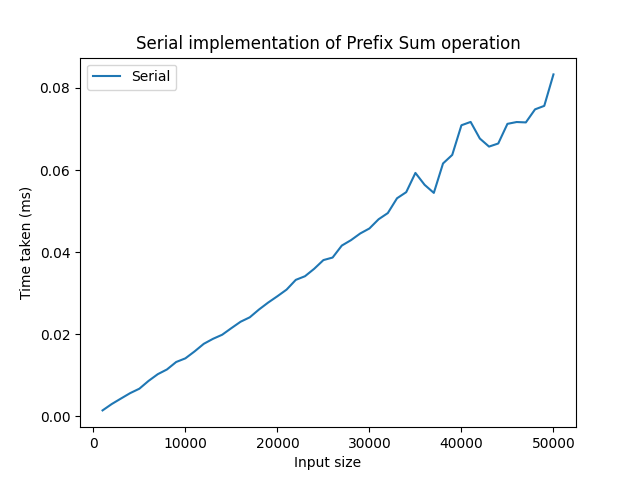
\includegraphics[width=0.6\linewidth]{serial_scan.png}
		\caption{Serial scan operation average times}
		\label{fig:fig_serial_scan}
	\end{figure}
	
	\newpage
	\subsection{OpenMP Parallel Implementation:}
	Next I implented the scan operation within OpenMP's interface. The algorithm I used is based off the Blelloch\cite{Prefixsumwiki} work-effecient algorithm given in Listing~\ref{listing:ls_scan_omp}
	\begin{lstlisting}[caption={OpenMP Parallel algorithm for computing scan operation\cite{PrefixsumCSE}.}, label={listing:ls_scan_omp}]
		void scan(int out[], int in[], int N){
			int nthr, *z, *x = out;
			#pragma omp parallel num_threads(4)
			{
				int i;
				#pragma omp single
				{
					nthr = omp_get_num_threads();
					z = malloc(sizeof(int)*nthr+1);
					z[0] = 0;
				}
				
				int tid = omp_get_thread_num();
				int sum = 0;
				#pragma omp for schedule(static)
				for(i=0; i<N; i++) {
					sum += in[i];
					x[i] = sum;
				}
				
				z[tid+1] = sum;
				#pragma omp barrier
				
				int offset = 0;
				for(i=0; i<(tid+1); i++) {
					offset += z[i];
				}
				
				#pragma omp for schedule(static)
				for(i=0; i<N; i++){
					x[i] += offset;
				}
			}
			free(z);
		}
	\end{lstlisting}

	The algorithm works as follows:
	\begin{itemize}
		\item Start omp parallel
		\item Initiate a 'single' construct which allows only one thread to run the code
		\item Inside single should declare the size of the temp array and set $element[0] = 0$
		\item After the single construct, get current threadID and initialize $sum =0$
		\item Begin an omp for contruct with schedule(static)
		\item Inside the for loop (from $0$ to $N-1$), $sum +=$ the input array at $i$, and set the output array at $i$ equal to the new $sum$
		\item After the for loop, set temp array at $[threadID+1]$ equal to $sum$
		\item Declare a Barrier construct which forces all threads to wait until other threads finish computation
		\item Set offset $= 0$ 
		\item Begin a regular for loop that sums all elements of the temp array to $offset$, only adding elements that each specific thread has computed itself
		\item Begin an omp for construct with schedule(static) again, from $i = 0$ to $N-1$
		\item sum output array element $i$ with offset
		\item Finish off pragma omp and then free the temp array from memory
	\end{itemize}
	
	I experimented with different number of threads running and managed to narrow it down to thread counts of $2,4,6$ given in Figure~\ref{fig:fig_scan_omp_comparison}
	
	With 2 threads running there is no noticeable speedup compared to serial implementation. With 4 and 6 threads running there is significant speedup compared to serial implementation. While input size n increases, 4 threads performs slightly better than 6 threads. Thus I choose 4 threads as my optimal implementation of OpenMP parallelization.
	\begin{figure}[!htb]
		\centering
		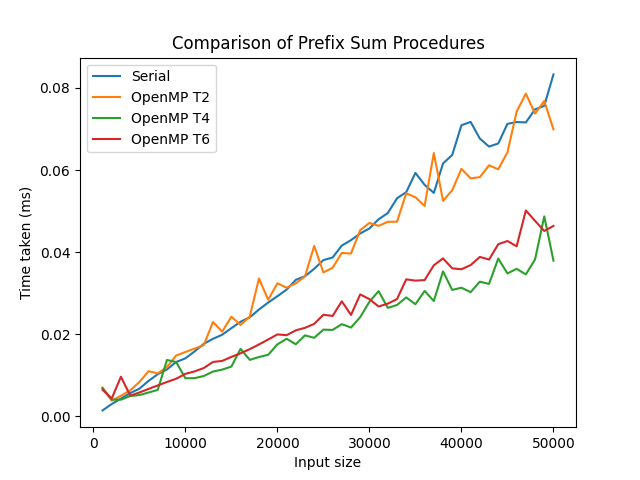
\includegraphics[width=0.6\linewidth]{scan_omp_comparison.png}
		\caption{OpenMP Parallel scan operation average times for different thread counts}
		\label{fig:fig_scan_omp_comparison}
	\end{figure}
	
	\subsection{MPI Parallel Implementation:}
	Next I implented the scan operation within MPI's interface. The algorithm I used is based off the Blelloch\cite{Prefixsumwiki} prescan algorithm given in Listing~\ref{listing:ls_scan_mpi}
	\begin{lstlisting}[caption={MPI Parallel algorithm for computing scan operation\cite{PrefixsumMPI}.}, label={listing:ls_scan_mpi}]
		MPI_Init(&argc, &argv); //Initialize MPI
		
		MPI_Comm_rank(MPI_COMM_WORLD, &my_rank);
		MPI_Comm_size(MPI_COMM_WORLD, &comm_size);
		
		MPI_Barrier(MPI_COMM_WORLD);
		
		size_t num_per_proc = n / comm_size;
		int sum;
		
		start_find_sum(my_rank, comm_size, data, num_per_proc,
		&sum);
		start_find_psum(my_rank, comm_size, data, num_per_proc,
		sum);
		
		MPI_Barrier(MPI_COMM_WORLD);
		
		MPI_Finalize(); //Close MPI
	\end{lstlisting}
	
	The essence of the algorith comes from the start\textunderscore find\textunderscore sum() and start\textunderscore find\textunderscore psum() functions.
	
	The algorithm works as follows:
	\begin{itemize}
		\item Start MPI
		\item Get comm rank and size
		\item Barrier that forces all threads to wait
		\item Set num per proc equal to array size $n / comm size$. This dictates how many numbers each thread will compute the sums of
		\item Call start\textunderscore find\textunderscore sum() function
		\begin{itemize}
			\item The algoritem works like a binary tree with levels
			\item Gets MPI\textunderscore Status
			\item Sums input array elements from $0$ to $numPerProc$
			\item Begin for loop from $level =0$ to $log_{2}(comm size)$
			\item Inside the loop set $position = rank / level^{2}$
			\item If $position$ is even, receives the $sendersSum$ (with $senderRank = rank + level^2$) and adds to total $sum$
			\item If $position$ is odd, sends total $sum$ to receiver with $senderRank = rank - level^2$, then kills current thread
			\item Before for loop ends, calls Barrier so all threads wait
		\end{itemize}
		\item Call start\textunderscore find\textunderscore psum() function
		\begin{itemize}
			\item The algorithm works like a binary tree with levels
			\item Gets MPI\textunderscore Status
			\item If $rank == 0$, sets $psum = sum$
			\item Begin for loop from $level = log_2(comm size) -1$ down to $0$
			\item If process is on current level:
			\item Set $position = rank / level^2$
			\item If $position$ is even this means this process was the parent of $sendingRank$, and so first sets $senderRank = rank + level^2$, then sends $psum$, then receives the $senderSum$ and finally subtracts $psum$ by $senderSum$
			\item If $position$ is odd, sets $receivingRank = rank - level^2$, then receives $psum$ from parent, and then sends $sum$ with $receivingRank$
			\item Before for loop ends, calls Barrier so all threads wait
			\item After the loop ends, put the $prefixSums$ associated with this process in the input array
		\end{itemize}
		\item Calls Barrier so all threads wait
		\item Ends MPI
	\end{itemize}
	
	With start\textunderscore find\textunderscore sum() and start\textunderscore find\textunderscore psum() functions given respectively by Listing~\ref{listing:ls_findsum} and Listing~\ref{listing:ls_findpsum}
	\begin{lstlisting}[caption={start\textunderscore find\textunderscore sum()}, label={listing:ls_findsum}]
		void start_find_sum(int rank, int mysize, int* in, 
							size_t num_per_proc, int* overall_sum){
			MPI_Status status;
			
			int sum = find_sum(in, num_per_proc);
			
			int still_alive = 1;
			int level;
			
			for (level = 0; level < (int)log2(mysize); level++) {
				if (still_alive) {
					int position = rank / (int)pow(2, level);
					
					if (position % 2 == 0) {
						// I am a receiver
						int sender_sum;
						int sending_rank = rank + (int)pow(2, level);
						
						MPI_Recv(&sender_sum, 1, MPI_INT, sending_rank,
						0, MPI_COMM_WORLD, &status);
						
						sum += sender_sum;
					}else {
						// I am a sender
						int receiving_rank = rank - (int)pow(2, level);
						
						MPI_Send(&sum, 1, MPI_INT, receiving_rank, 0,
						MPI_COMM_WORLD);
						still_alive = 0;
					}
				}
				MPI_Barrier(MPI_COMM_WORLD);
			}
			*overall_sum = sum;
		}
	\end{lstlisting}
	\begin{lstlisting}[caption={start\textunderscore find\textunderscore psum()}, label={listing:ls_findpsum}]
		void start_find_psum(int rank, int mysize, int* in,
							size_t num_per_proc, int sum){
			int psum;
			int level;
			MPI_Status status;  
			
			if (rank == 0) {
				psum = sum;
			}
			for (level = (int)log2(mysize) - 1; level >= 0; level--) {
				// only trigger the processes on the current level
				if (level == 0 || rank % (int)pow(2, level) == 0) {
					int position = rank / (int)pow(2, level);
					
					if (position % 2 == 0) {
						int sender_sum;
						int sending_rank = rank + (int)pow(2, level);
						
						MPI_Send(&psum, 1, MPI_INT,
						sending_rank, // RIGHT CHILD
						0, MPI_COMM_WORLD);
						
						MPI_Recv(&sender_sum, 1, MPI_INT,
						sending_rank, 0, MPI_COMM_WORLD, &status);

						// psum <- (prefix sum of parent) - (sum of sibling)
						psum -= sender_sum;
					}else{
						int receiving_rank = rank - (int)pow(2, level);
						
						MPI_Recv(&psum, 1, MPI_INT,
						receiving_rank, // PARENT
						0, MPI_COMM_WORLD, &status);
						
						// send sum to receiving_rank so it can fix its sum
						MPI_Send(&sum, 1, MPI_INT,
						receiving_rank, 0, MPI_COMM_WORLD);
					}
				}
				MPI_Barrier(MPI_COMM_WORLD);
			}
			// put the prefix sums associated with this node in input array
			int next_sum = in[num_per_proc-1];
			in[num_per_proc-1] = psum;
			
			for (int j = num_per_proc - 2; j >= 0; j--) {
				int next_sum_tmp = in[j];
				
				in[j] = in[j+1] - next_sum;
				
				next_sum = next_sum_tmp;
			}
		}
	\end{lstlisting}
	
	I experimented with different number of threads running and managed to narrow it down to thread counts of $2,4,8$ given in Figure~\ref{fig:fig_scan_mpi_comparison}
	
	With 2 threads running there is noticeably worse running time compared to serial implementation. With 4 and 8 threads running there is significant speedup compared to serial implementation. With smaller input sizes n, 4 threads performs better than 8 threads, but as n increases, perfermance between 4 threads and 8 threads stays relatively the same. Thus I choose 4 threads as my optimal implementation of MPI parallelization.
	\begin{figure}[!htb]
		\centering
		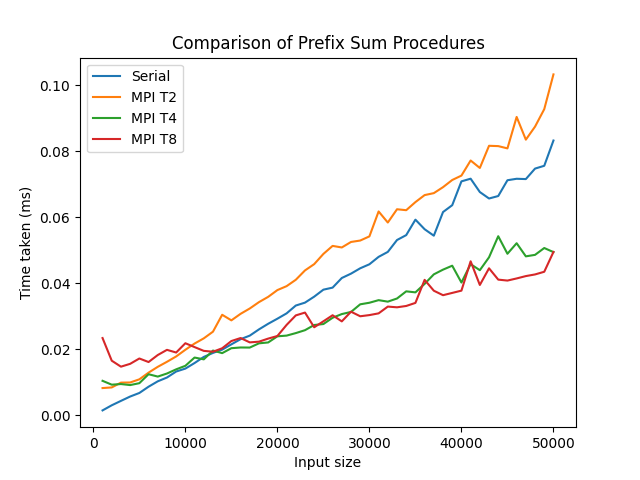
\includegraphics[width=0.6\linewidth]{scan_mpi_comparison.png}
		\caption{MPI Parallel scan operation average times for different thread counts}
		\label{fig:fig_scan_mpi_comparison}
	\end{figure}

	\subsection{Validation:}
	Checking if elements are correclty summed, through running $run.sh$ given in Figure~\ref{fig:fig_validation}
	\begin{figure}[!htb]
		\centering
		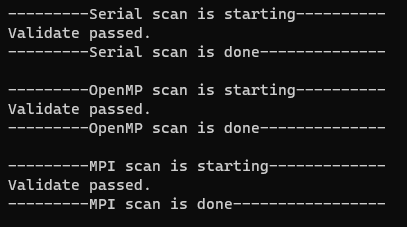
\includegraphics[width=0.5\linewidth]{validation.png}
		\caption{Validation of scan operations}
		\label{fig:fig_validation}
	\end{figure}

	\subsection{Conclusions:}
	After comparing the results from serial, optimal OpenMP (with 4 threads) and optimal MPI (with 4 threads), I can make the conclusion that serial performs the best at very small array size n. While at large n, both OpenMP and MPI have significant speedup from serial, OpenMP performs consistently better than MPI.
	Comparisons given in Figure~\ref{fig:fig_scan_comparison}
	\begin{figure}[!htb]
		\centering
		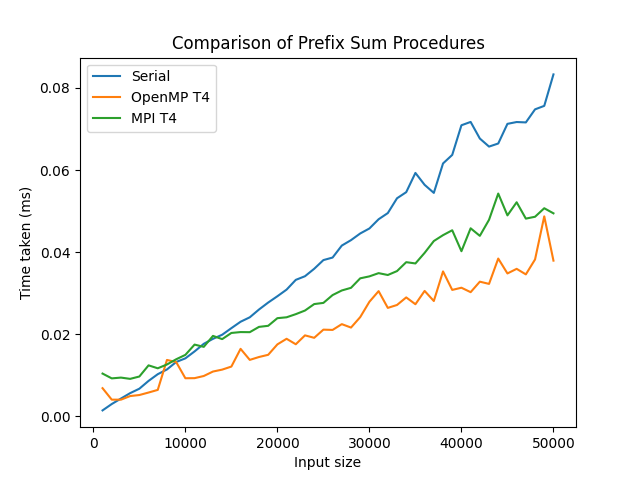
\includegraphics[width=0.6\linewidth]{scan_comparison.png}
		\caption{Comparison of all scan operations}
		\label{fig:fig_scan_comparison}
	\end{figure}

	\section{Problem 2: Parallel Bitonic Sort}
	Not applicable, working alone.
	
	\section{Problem 3: Parallel Graph Algorithm}
	Implementing Dijkstra’s Single Source Shortest Path (SSSP) Algorithm. An example problem is given in Figure~\ref{fig:sp_fig1}.
	\begin{figure}[!htb]
		\centering
		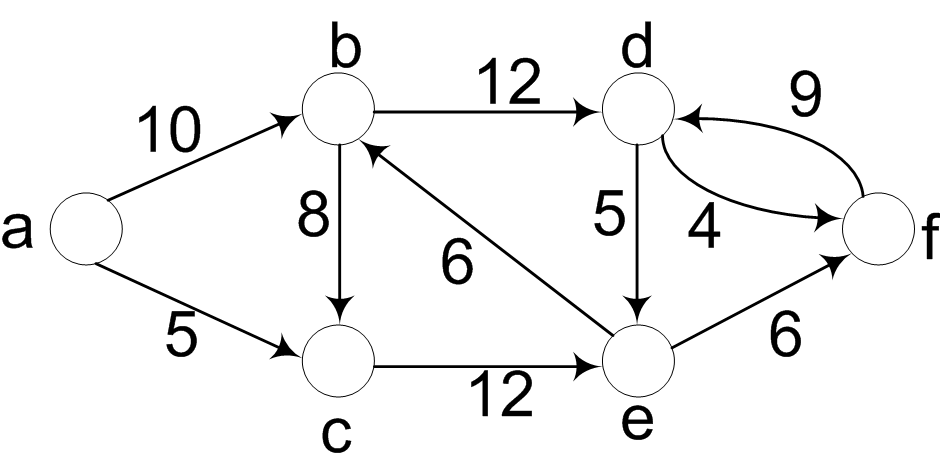
\includegraphics[width=0.3\linewidth]{sp_fig1.png}
		\caption{A directed graph}\label{fig:sp_fig1}
	\end{figure}
	
	\subsection{Serial Implementation:}
	Firstly I started off with the baseline implementation of serial SSSP algorithm given in Listing~\ref{listing:ls_serial_sssp}
	\begin{lstlisting}[caption={Sequential algorithm for Dijkstra’s SSSP\cite{SSSP}.}, label={listing:ls_serial_sssp}]
		int* dijkstra(int **graph, int src){
			int* dist = (int*)malloc(V * sizeof(int));
			bool sptSet[V]; 

			for (int i = 0; i < V; i++) dist[i] = INT_MAX, sptSet[i] = false;
			dist[src] = 0;
			
			// Find shortest path for all vertices
			for (int count = 0; count < V - 1; count++) {
				int u = minDistance(dist, sptSet);
				sptSet[u] = true;

				for (int v = 0; v < V; v++)
					if (!sptSet[v] && graph[u][v] && dist[u] != INT_MAX
					&& dist[u] + graph[u][v] < dist[v])
					dist[v] = dist[u] + graph[u][v];
			}
			return dist;
		}
	\end{lstlisting}
	
	This got me a baseline average time to measure and compare parallel implementations. I ran the algorithm on the given graphs (15 times, taking average) with number of vertices ranging from $6$ to $512$ given in Figure~\ref{fig:fig_serial_sssp}
	\begin{figure}[!htb]
		\centering
		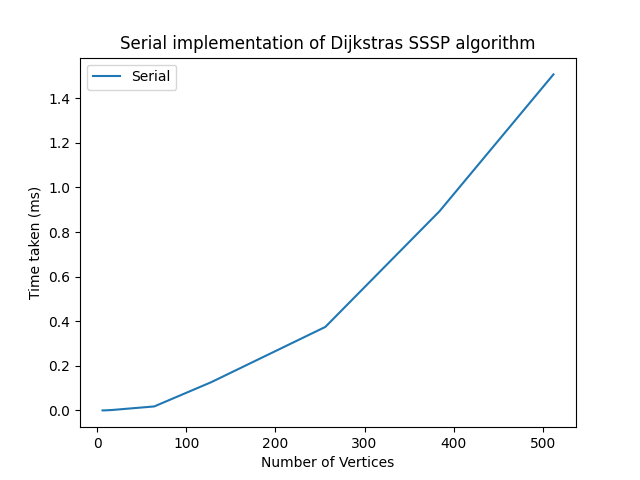
\includegraphics[width=0.6\linewidth]{serial_sssp.png}
		\caption{Serial SSSP algorithm average times}
		\label{fig:fig_serial_sssp}
	\end{figure}

	\newpage
	\subsection{Conclusions:}
	An example of table is given Table~\ref{tab:example}.
	\begin{table}[!htb]
		\centering
		\caption{An example of a table}\label{tab:example}
		\begin{tabular}{l|ccccc}
			\toprule
			No of vertices & 64 & 128 & 256 & 384 & 512\\
			\midrule
			Serial &0.1&0.2&0.3&0.4&0.5\\
			Parallel &&&&\\
			Sppedup &2&3&4&5&6\\
			\bottomrule
		\end{tabular}
	\end{table} 
	
	\newpage
	\bibliography{main}
	
\end{document} 

